%%%%%%%%%%%%%%%%%%%%%%%%%%%%%%%%%%%%%%%%%%%%%%%%%%%%%%%%%%%%%%%%%%%
%                                                                 %
%                            CHAPTER                              %
%                                                                 %
%%%%%%%%%%%%%%%%%%%%%%%%%%%%%%%%%%%%%%%%%%%%%%%%%%%%%%%%%%%%%%%%%%%

\NewDocumentCommand{\codeword}{v}{%
\texttt{\textcolor{blue}{#1}}%
}

\chapter{Implementation}
In this chapter we will explain how we implemented MPC for face matching algorithms. We will do this by giving a high-level overview of the system and then diving deeper in more interesting parts. With this information and the code in the appendix, you should be able to reproduce our experiments. You can also checkout our Github repository\footnote{\url{github.com/Fluxmux/securefacematching}}.
%TODO: Phrase this better

\section{Specifications}
There are two major subprojects. The first subproject (chapter \ref{Deep Learning}) is making sure we can generate the appropriate parameters for the face matching network. It is important that the model is accurate enough. The second subproject (chapter \ref{Secure Functions}) is about transforming the classic machine learning functions to secure ones. To add this security or privacy-preserving factor we use a MPC framework.

\subsection{Deep Learning}
\label{Deep Learning}
A machine learning project usually includes on of the popular frameworks available to the public. Since we were already familiar with Pytorch we used this library as a python package.

Pytorch \footnote{\url{pytorch.org}} provides us with a deep learning research platform that provides maximum flexibility and speed. It's fairly easy to use but that doesn't mean we can't design more complex models or features. Pytorch uses tensors, tensors are multi-dimensional matrix containing elements of a single data type. Designing a neural network with Pytorch is as simple as defining a class with the layers in the correct order. An example of a neural network written using pytorch can be seen in the following code (listing~\ref{lst:pytorch_example})\\

\begin{lstlisting}[language=Python, caption={Pytorch neural network example}, label={lst:pytorch_example}, frame=single]
class SiameseNetwork(nn.Module):
    def __init__(self):
        super(SiameseNetwork, self).__init__()

        self.cnn = nn.Sequential(
            nn.ReflectionPad2d(1),
            nn.Conv2d(1, 16, kernel_size=5),
            nn.ReLU(inplace=True),
            nn.BatchNorm2d(16),
            nn.MaxPool2d(kernel_size=2, stride=2),
            ...
        )
\end{lstlisting}

Making an accurate face matching neural network. Is a process that involves three major steps.

First of all the design or architecture of the network gets chosen. There exist a number of different topologies used in deep neural networks. But often choosing which one to take and how many layers to use, is the most difficult task. We will cover the architecture of the model in chapter \ref{Design}. Adding more layers is the same as adding more parameters. And a model with more parameters is more complex.

The second step is called the traing of the neural network. Training is done using a part of the dataset that is specific for training and shouldn't be used for anything else.

A typical workflow of the training step looks something like this: Two labeled faces are sent seperatly sent through the network. The euclidean distance (equation \ref{eq:euclideandistance}) for inputs $\vec{X_{1}}$ and $\vec{X_{2}}$ and the parameterized function $G_{W}$ calculates the distance between the outputs. This distance metric should be close to zero for faces belonging to the same person. But as large as possible for faces belonging to different person.

\begin{equation} \label{eq:euclideandistance}
  D_{W}(\vec{X_{1}},\vec{X_{2}})=\lVert G_{W}(\vec{X_{1}}) - G_{W}(\vec{X_{2}}) \rVert
\end{equation}

Then we use the loss function Yann LeCun first introduced in his paper \cite{hadsell2006dimensionality}; The general loss function $L$ is the sum of contrastive loss functions for a training pair in the set of training pairs of size $P$.

Let $Y$ be the binary label assigned to this pair of faces, $Y=0$ if $\vec{X_{1}}$ and $\vec{X_{2}}$ are labeled as similar, and $Y=1$ if $\vec{X_{1}}$ and $\vec{X_{2}}$ are labeled as dissimilar.

\begin{equation} \label{eq:contrastiveloss}
  L(W,Y,\vec{X_{1}},\vec{X_{2}})=(1-Y)\frac{1}{2}(D_{W})^{2} + Y\frac{1}{2}(max^{2}(0, m - D_{W}))
\end{equation}

The contrastive loss function is definded in formula \ref{eq:contrastiveloss}, where $m > 0$ is the margin. The margin $m$ can be seen as a radius so that dissimilar pairs still contribute to the loss function if their distance is withing this radius. The goal of training is to minimize the loss. For similar pairs this means decreasing the distance $D_{W}$, for dissimilar pairs this means increasing the distance to be greater than the margin. We came to the conclusion that our loss reduces the most if we choose a margin of $m=2$.

We also tried a different approach, instead of using this distance metric (which we would than have to statically threshold) we would like to have a probability value between $0$ and $1$. The output layer of the network consists out of two neurons (two classes), one neuron describes the similar faces, the other neuron describes the dissimilar faces. A probability of $0$ means that the faces belong to different persons and a probability of $1$ means that the faces belong to the same person. Binary Cross Entropy loss, or Logaritmic loss (equation \ref{eq:crossentropyloss}) is one of the loss functions that can be used to achieve this.

\begin{equation} \label{eq:crossentropyloss}
  L=-{(y\log(p) + (1 - y)\log(1 - p))}
\end{equation}

Let $y$ be the binary label assigned to this pair of faces, $p$ is the predicted probability. To visualize this loss function, have a look at figure \ref{fig:crossentropyloss}

\begin{figure}[H]
  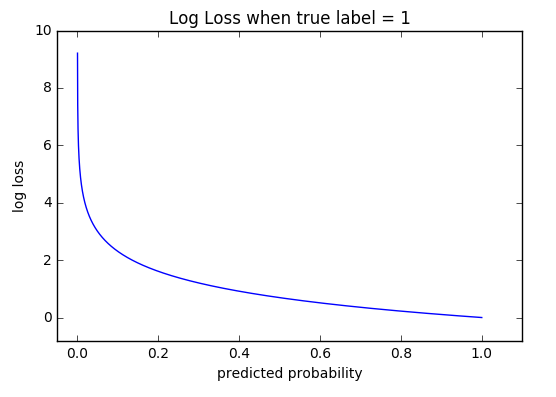
\includegraphics[scale=0.6]{fig/cross_entropy.png}
  \centering
  \caption{Range of loss values for $y=1$}
  \label{fig:crossentropyloss}
\end{figure}

There exist a great number of other functions. Some might be better suited for the face matching problem. But since we need to keep things simple in order to implement MPC. We opt for one of the two loss functions described above.

Training a neural network takes some time, but the process can be sped up by using graphics processing units (GPU). We were lucky enough to have a dedicated GPU server at our disposal. While training the network is an easy task, we should look out for overfitting or underfitting.

Overfitting a model happens when there are too much parameters for a model or when the training was performed for too long. It will perform poorly on the validation dataset (part of dataset used to detect bad trainig behaviour) while performing excellent on the training dataset. There are two ways of overcoming overfitting. One way is to make the training dataset larger. Having more samples to train on, generalizes the learning model better. The other way is to design the model with fewer parameters, making it less complex. We use learning curves to track the training process of our face matching algortihm. An example of a more or less correct learning curve can be found in figure \ref{fig:trainingcurve}.

\begin{figure}[H]
  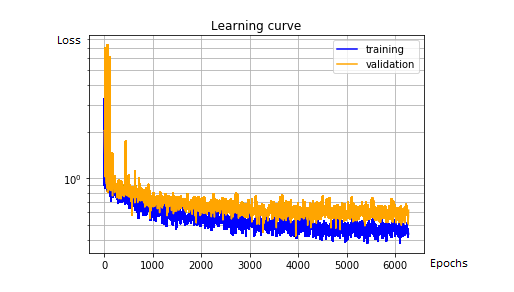
\includegraphics{fig/trainingcurve.png}
  \caption{Learning curves are used to track the training of a model}
  \label{fig:trainingcurve}
\end{figure}

Underfitting happens when a machine learning algorithm cannot capture the underlying structure of data. The model can't fit the data enough. Underfitting is more difficult to spot but easier to overcome. We can overcome this problem by making our model more complex.

As you can see by now, the architecture of a model is extremely important for it to function as wished.

The third step also called the hyperparameter tuning or hyperparameter optimisation step, is what makes a good machine learning model even better. This process is not at all logic, experience and intuition can facilitate this. Hyperparameters are all the parameters whose values are set before the learning process begins. There are different methods for optimizing hyperparameters, since we wanted to learn the model and how it behaves relating to small changes in the values of the hyperparameters we went for Manual Random Search. Note that this took us some time because this involves multiple training steps. But since we had a GPU server at our disposal we could parallelize this task. In our case this step improved our accuracy by about 5\%.

We used the Database of Faces\footnote{\url{cam-orl.co.uk/facedatabase.html}} to train and test our face matching algortihm. The dataset contains a set of 10 images of frontal faces with different expressions per person and a total of 40 persons. The pictures are in pgm format which is extremely easy to interact with. They have a dimension of 1 x 92 x 112. An example of a set of images from the dataset can be seen in figure \ref{fig:databaseoffaces}. We divided the dataset in to 3 parts: 75\% training, 12.5\% testing and another 12.5\% for validation.

\begin{figure}[H]
  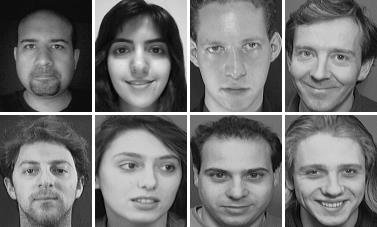
\includegraphics[scale=0.7]{fig/databaseoffacess.png}
  \centering
  \caption{Example of faces in dataset}
  \label{fig:databaseoffaces}
\end{figure}

\subsection{Secure Functions}
\label{Secure Functions}
Secure functions or the privacy preserving equivalent of an ordinary function can be used to compute an encrypted output as a function of encrypted inputs (figure \ref{fig:blackbox}). The protocol used for defining these secure functions is the MPC protocol.

\begin{figure}[H]
  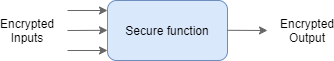
\includegraphics[scale=0.8]{plots/blackbox.png}
  \centering
  \caption{Secure function as a black box}
  \label{fig:blackbox}
\end{figure}

Berry Schoenmakers is a cryptographer working on cryptographic protocols for electronic voting, electronic payments and secure multiparty computation. Since 2018 he has been working on a general MPC implementation for python, called MPyC. This pyhton package can be easily installed with pip: \codeword{pip install mpyc}. For more information on how to use this package have a look at the source code at \url{github.com/lschoe/mpyc}.

There are number of basic functions predefined, like \keyword{add}, \keyword{sub}, \keyword{mul} and \keyword{div}, respectively $+$, $-$, $\times$ and $\div$. As well as \keyword{eq} (equal to), \keyword{ge} (greater than or equal), \keyword{min} and \keyword{max}. The total set of available functions can be found in \keyword{mpyc.runtime.py}. But for our task the functions noted above are all we need.

With this set of fundamental functions we can generate our own custom functions that serve our needs. We introduce three essential custom secure functions that can be found in \keyword{/mpc/device/mpyc/demo/custom_operations.py}.

\begin{itemize}
  \item \keyword{convolution}.
  \item \keyword{maxpooling}.
  \item \keyword{relu}.
\end{itemize}


\section{Design}
\label{Design}


\section{Conclusion}
